\documentclass[10pt,twocolumn]{article}
\usepackage[margin=0.9in]{geometry}
\usepackage{amsmath,amssymb}
\usepackage{graphicx}
\usepackage{booktabs}
\usepackage{hyperref}
\usepackage[numbers]{natbib}

\title{Heterogeneous Role Allocation Under Partial 3D Observability and
Dynamic Connectivity in Counter-Drone Swarm Defense}
\author{Arav Kaul}
\date{July 2026}

\begin{document}
\maketitle

\begin{abstract}
We simulate a drone-versus-drone defense problem in full 3D. A team of
sixteen defenders protects a site against a swarm of up to sixteen evasive
attackers. The defenders are split into three roles: slow, high-flying
\emph{sentinels} that carry the wide-area sensors; fast
\emph{interceptors} that chase targets with a 3D missile-guidance law; and
\emph{relays} whose only job is to keep the team's wireless mesh connected.
The three usual subproblems---assigning pursuers to targets, tracking
targets through occlusion, and keeping the network connected---are simulated
together rather than separately: target assignments can only be agreed among
drones that can currently communicate, sensors are blocked by buildings, and
a sprinting interceptor physically breaks the network that feeds it target
updates. Across attack sizes of 4--16 (10 random seeds each), the specialist
team detects attackers 2.6--3.1\,s sooner than a same-size team of identical
``generalist'' drones, and this earlier detection accounts for its lower mean
time-to-intercept at every attack size (significant against 4 and 8
attackers, not against 12 and 16). Relays raise the network's algebraic
connectivity $\lambda_2$ 2.1--2.3$\times$ over a same-size team that spends
those airframes on interceptors, and 3.8$\times$ after 3 of the 16 defenders
are destroyed, but part of this gain is built into the metric, and we find no
measurable gain in how often the network is fully connected or in
interception rate. At this scale, the simulated benefit of a dedicated relay
role is smaller than the coupled-system framing suggests; the benefit of
dedicated sensing is clear.
\end{abstract}

\section{Introduction}
Defending a site against a swarm of small, fast drones is hard for one
simple reason: no single aircraft is good at everything. A platform built to
see far must fly high and slow. A platform built to chase must be fast and
burns through its battery. A platform in the right place to relay messages
is usually in the wrong place to do anything else. So a natural design is a
\emph{heterogeneous} team---different aircraft for different jobs.

But splitting the jobs creates a coordination problem, and that problem
lives or dies on communication. In our setting, nothing is globally known:

\begin{itemize}
\item \textbf{Seeing is geometric.} Sensors cover cones and spheres of 3D
space and are blocked by buildings. Attackers exploit this by flying low
among the buildings, appearing and disappearing from view.
\item \textbf{Talking is geometric too.} Radio links need both range and a
clear line of sight, and get lossier with distance. The network's shape
changes every second as drones move.
\item \textbf{Coordination rides on talking.} The auction that decides which
interceptor chases which attacker can only run among drones that can
currently reach each other. An interceptor that sprints 500\,m after a
target may cut itself off from the very sentinels that are tracking it.
\end{itemize}

The question we study: \emph{when the team's own motion constantly reshapes
what it can see and say, what does each role actually buy you?} We answer it
by simulation, comparing the specialist team against two same-size baselines
that spend the same sixteen airframes differently.

\section{Related Work and Gap}
Each ingredient of this problem has its own mature literature. Market-based
task allocation---notably the consensus-based bundle algorithm (CBBA) and
its descendants---assigns robots to tasks without a central
computer~\cite{cbba,mrta_survey}, but its guarantees assume the network is
connected. Connectivity maintenance controls a network's \emph{algebraic
connectivity} $\lambda_2$, a standard graph-theoretic measure of how far a
network is from splitting, and moves robots to keep it
high~\cite{zavlanos,uav_relay_recovery}---but usually as a goal in itself,
not in service of a concurrent fight. Counter-drone swarm defense work,
often reinforcement-learning based, typically assumes identical defenders
and idealized communications~\cite{xuan2022,zhao2022,rl_prioritization}.

The gap is the coupling. Allocation papers idealize the network;
network papers idealize the mission; defense papers idealize both. What is
missing is a closed-loop account of \emph{heterogeneous role allocation
under partial 3D observability and dynamic connectivity}: assignment that
only works where the network reaches, sensing that only works where
geometry allows, and relays that try to buy back the connectivity that
pursuit destroys. Our contribution is not a new algorithm but a quantified
account of how these pieces interact in one closed-loop simulation,
including where a role's expected benefit does and does not show up. The project extends the author's earlier 2D work
on adaptive communication topology to 3D, with occlusion and heterogeneous
roles.

\section{Method}
\subsection{Agents}
All aircraft are 3D point masses: position and velocity, with role-specific
caps on speed and acceleration (Table~\ref{tab:roles}), integrated at
50\,ms steps. Sentinels are slow, fly at 150\,m, and carry a
downward-looking cone sensor (450\,m range). Interceptors are fast
(42\,m/s) with a short-range seeker, and drain fuel with the square of
their speed (fuel never binds in our engagements; see
Section~\ref{sec:results}). Relays carry the long-range radios and no sensor. The
homogeneous baseline ``generalist'' is a compromise aircraft: mid speed,
mid sensor, no specialization.

\begin{table}[t]
\centering\small
\setlength{\tabcolsep}{3pt}
\begin{tabular}{lcccc}
\toprule
 & sentinel & interceptor & relay & generalist \\
\midrule
max speed [m/s] & 12 & 42 & 18 & 26 \\
max accel [m/s$^2$] & 4 & 28 & 8 & 13 \\
radio range [m] & 420 & 300 & 420 & 300 \\
sensor & cone $70^\circ$ & sphere & --- & sphere \\
sensor range [m] & 450 & 160 & --- & 300 \\
fuel [s at sprint] & $\infty$ & 100 & $\infty$ & 160 \\
\bottomrule
\end{tabular}
\caption{Role capability profiles.}
\label{tab:roles}
\end{table}

\subsection{Seeing and talking}
A detection requires the target to be inside the sensor's volume \emph{and}
visible along a straight 3D line not blocked by any of ten buildings
(50--130\,m tall) around the site. Detections yield noisy position and
velocity tracks that each drone stores locally. A radio link exists between
two drones when they are within range and have line of sight. Each tick,
every drone offers the tracks it held at the start of the exchange to each
neighbor, and each offer gets through with a probability that decays with
link distance, so a track advances at most one hop per 50\,ms tick. Information therefore spreads through the mesh
hop-by-hop---there is no global blackboard. Unrefreshed tracks are
extrapolated for up to 5\,s, then dropped.

\subsection{Deciding who does what}
Once per second, every connected group of drones runs a simple auction over
the fresh tracks it collectively holds (this is CBBA restricted to one task
per agent). Each interceptor with enough fuel bids its estimated
time-to-intercept, computed from the closing geometry; the lowest bid wins
each target, incumbents get a 20\% discount to prevent flip-flopping, and
spare interceptors double-team. An interceptor below the fuel gate drops
its task and returns to its ready point. A second auction assigns sentinels to four
fixed lookout stations on a ring above the site, weighted by where the
threats currently are. The key constraint is that both auctions run
\emph{per connected component}: a cut-off drone can only bid on the tracks
it already holds or senses itself.

\subsection{Chasing}
An assigned interceptor steers with proportional navigation (PN), the
classical missile guidance law, in its true 3D vector form. If
$\mathbf{r}$ is the vector to the target and $\mathbf{v}_{rel}$ the
relative velocity, the line of sight rotates at
$\boldsymbol{\Omega} = (\mathbf{r}\times\mathbf{v}_{rel})/\|\mathbf{r}\|^2$,
and the commanded acceleration
\[
\mathbf{a} = N\,\boldsymbol{\Omega}\times\mathbf{v}, \qquad N = 4,
\]
turns the interceptor so that the line of sight stops rotating---the
constant-bearing collision condition---while a second term holds sprint
speed. Passing within 6\,m scores a kill; interceptors are reusable
(net-capture style) and can be re-tasked after a kill.

\subsection{Keeping the network alive}
Relays climb the gradient of the network's algebraic connectivity
$\lambda_2$: using the graph Laplacian's Fiedler vector $\mathbf{f}$ (whose
entries split the network into its two most weakly joined halves), a relay
moves toward the neighbors whose $f$-values differ most from its own---that
is, toward the seam where the network would tear first. If the network has
already split, the relay flies to the midpoint of the shortest gap between
components. All defenders keep 15\,m separation via repulsive forces and
route around buildings the same way. Attackers approach at 15--35\,m
altitude among the buildings, weave continuously, and jink hard away from
any interceptor within 130\,m.

\section{Experimental Setup}
\label{sec:setup}
Attackers spawn 750--900\,m out in two clusters and win by reaching a
30\,m sphere around the site. All conditions field sixteen defenders:
\textbf{full} = 4 sentinels + 8 interceptors + 4 relays;
\textbf{no-relay} = 4 sentinels + 12 interceptors;
\textbf{homogeneous} = 16 generalists. Experiment E1 sweeps the attack size
$n\in\{4,8,12,16\}$; E2 fixes $n{=}8$ and destroys 3 random defenders at
$t{=}15$\,s. Every cell runs 10 seeds with a fixed building layout. We
report: interception rate; mean time-to-intercept (TTI), the time from the
start of the episode to the kill, averaged over killed attackers only;
mean first-detection time (when any defender's sensor first sees an
attacker) and mean time from first detection to kill; mesh uptime (the
fraction of time the whole team forms one connected network); mean
$\lambda_2$; largest-component fraction (LCF); and track coverage (the
fraction of live attackers the team currently holds a fresh track on).
TTI is dominated by approach geometry, since attackers spawn 750--900\,m
out, so only differences between teams are informative. Comparisons use
Welch's $t$-test over the 10 seeds.

Because the link weight $w=\exp(-(d/0.6R)^2)$ uses each link's radio range
$R$, $\lambda_2$ is not like-for-like across teams with different radios:
a relay--relay link at a given distance weighs more than an
interceptor--interceptor link. We therefore also report uptime and LCF,
which count only whether links exist.

Before any experiment, a verification gate checks that a single interceptor
converges on straight and evasive targets; that speeds and accelerations
recomputed from recorded positions stay within each role's limits, apart
from altitude-floor contacts (Section~\ref{sec:limits}); that swapping 4
interceptors for 4 relays at a fixed team size raises $\lambda_2$ on each of
10 paired seeds and raises mean uptime; and that buildings lower the mean
track coverage of low-flying attackers over 10 paired seeds. The last two
are direction checks, not significance tests; the occlusion effect is about
one percentage point.

\section{Results}
\label{sec:results}
\begin{figure}[t]
\centering
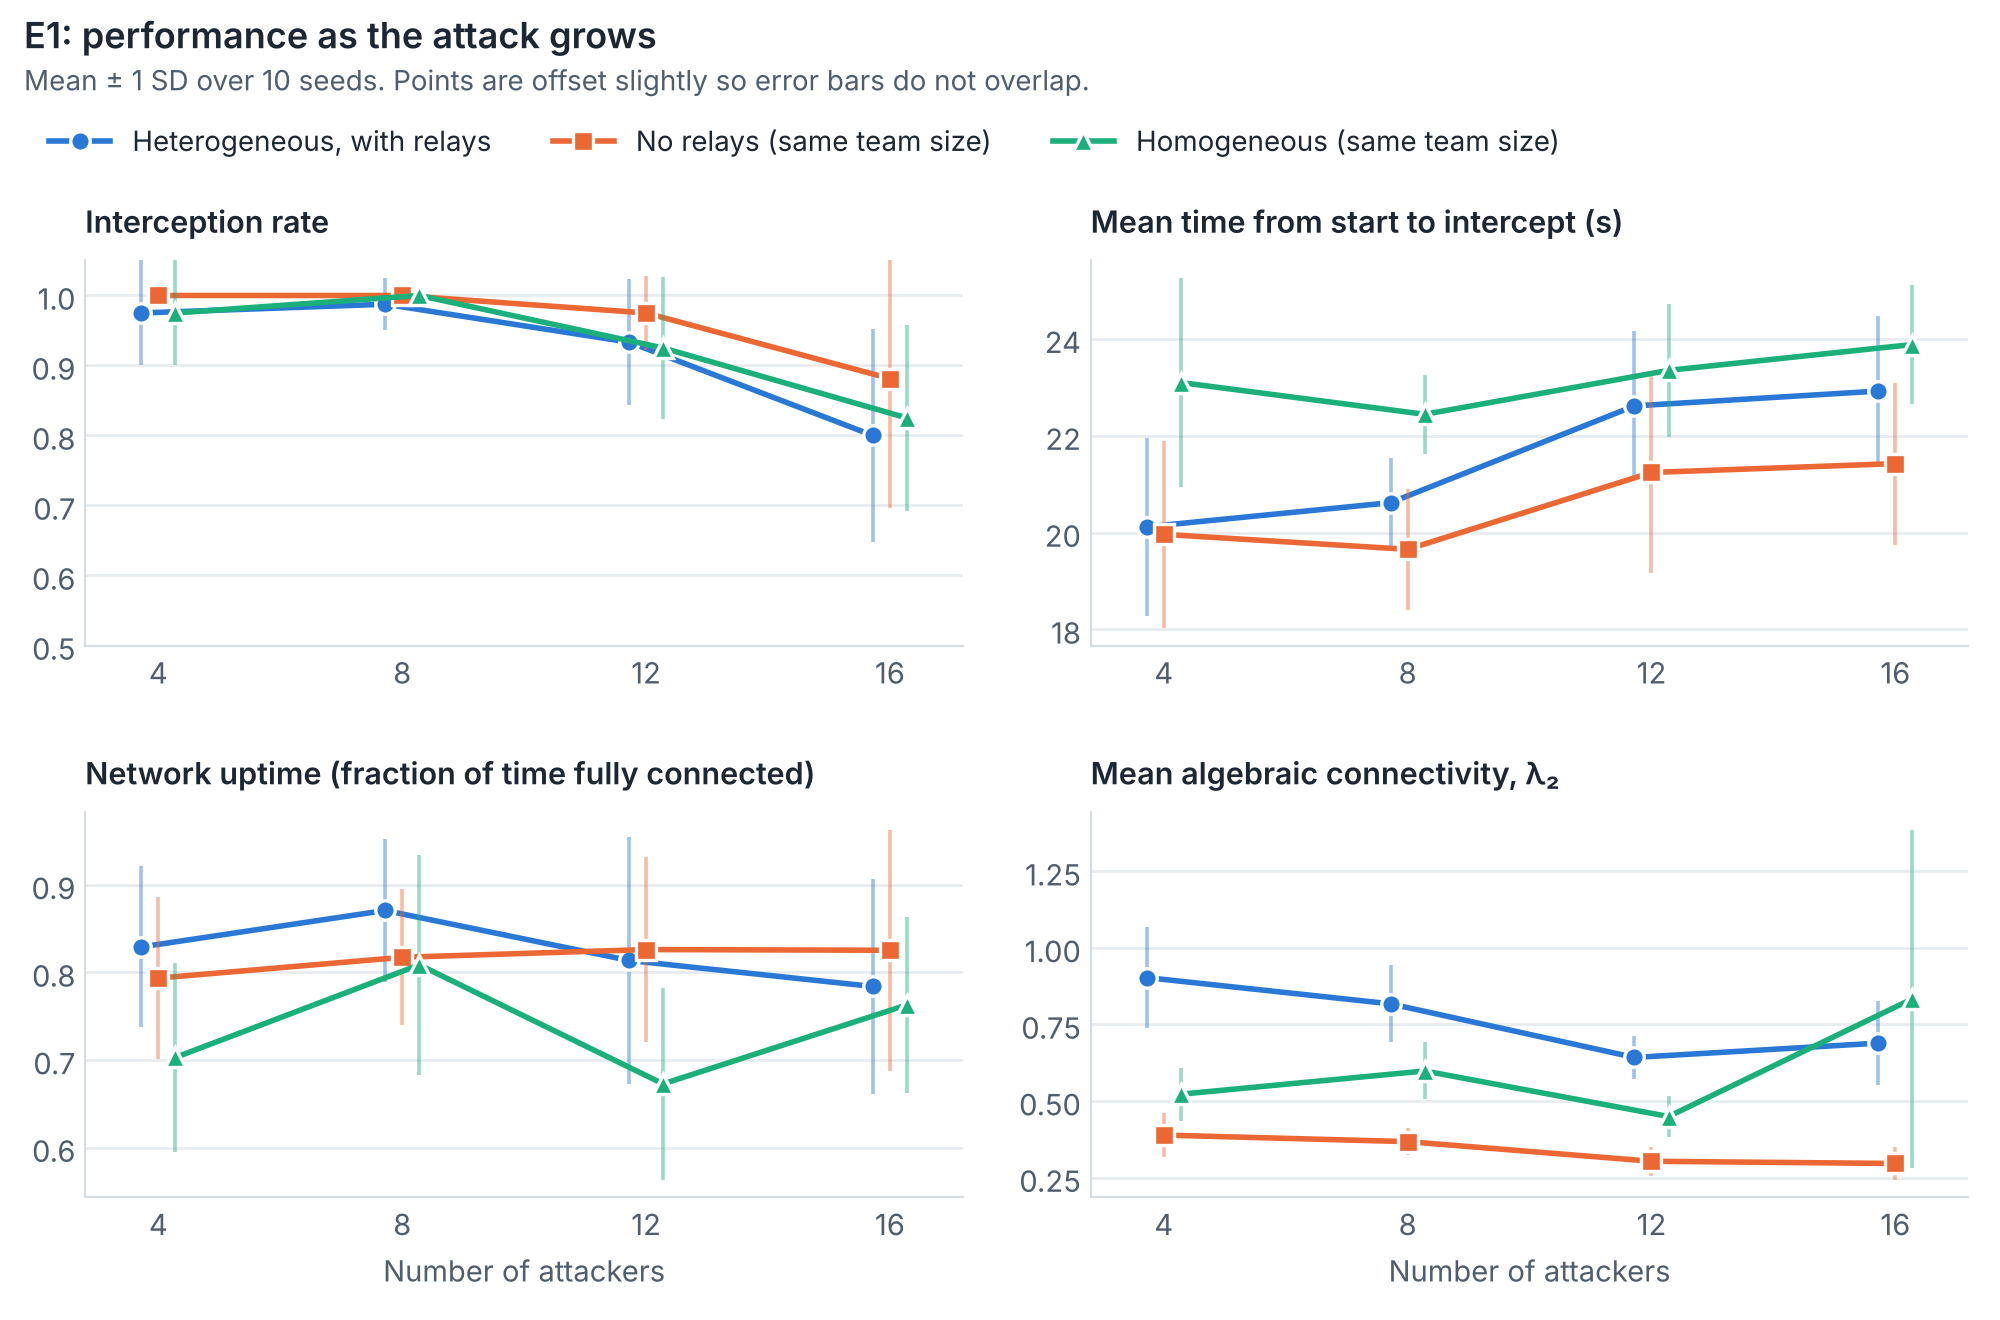
\includegraphics[width=\linewidth]{e1_scaling.png}
\caption{E1: scaling with threat swarm size (mean $\pm$ sd, 10 seeds).}
\label{fig:e1}
\end{figure}

\begin{figure}[t]
\centering
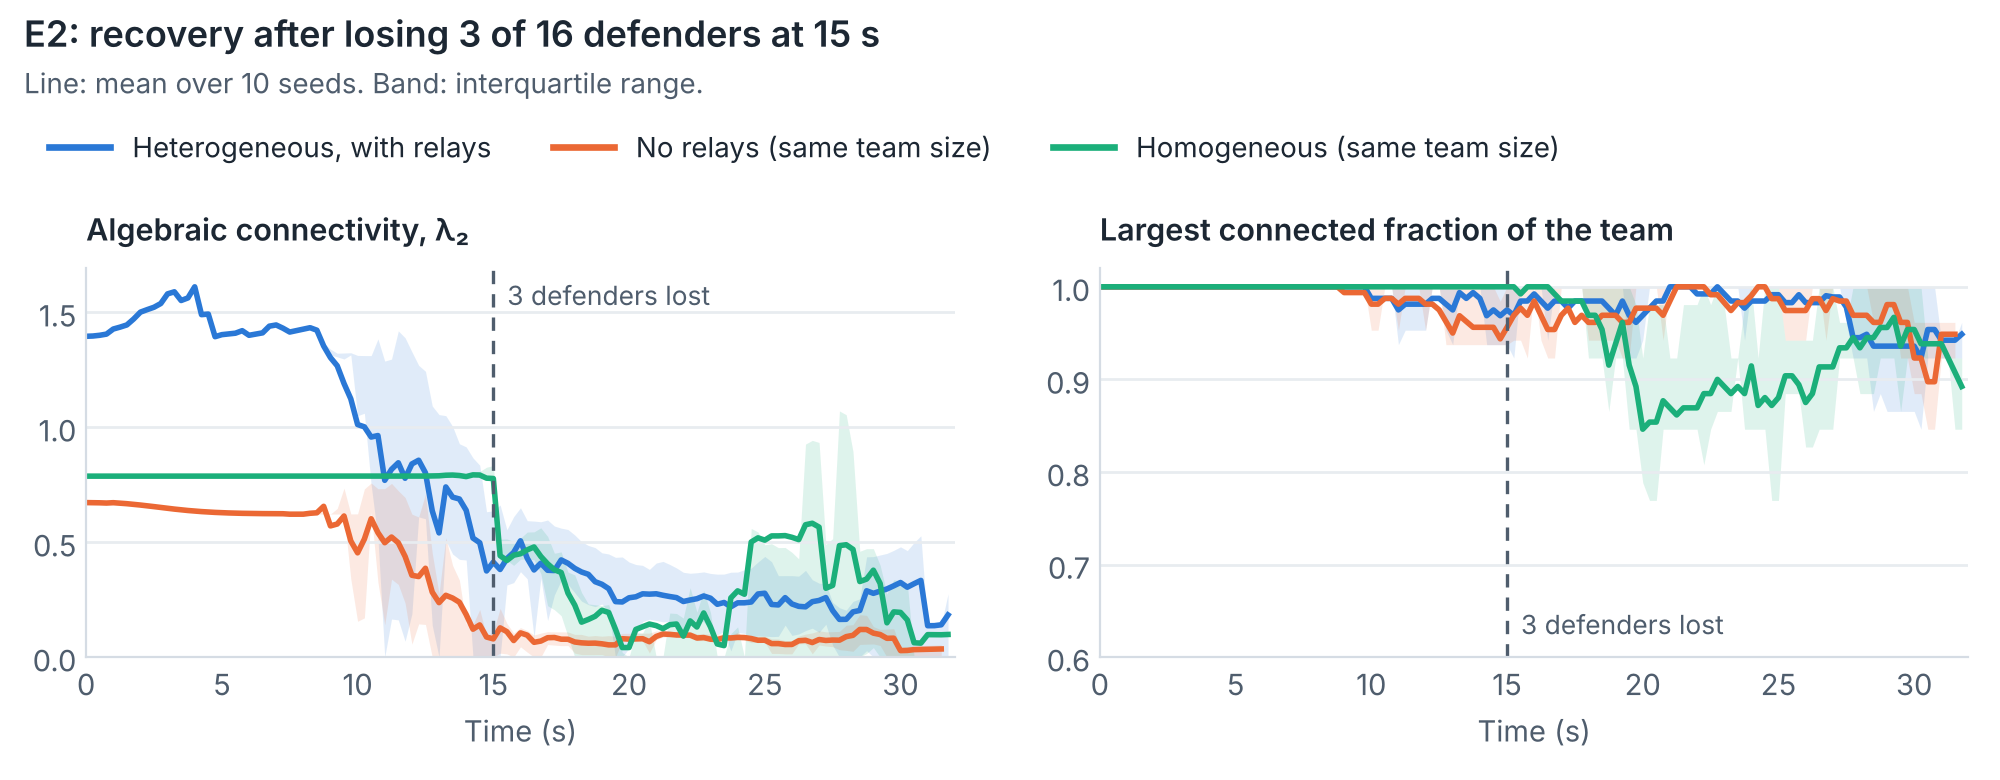
\includegraphics[width=\linewidth]{e2_resilience.png}
\caption{E2: connectivity before and after losing 3 of 16 defenders at
$t{=}15$\,s (line: mean over 10 seeds; band: interquartile range).}
\label{fig:e2}
\end{figure}

\textbf{Specialists detect earlier, and that is why they intercept
faster.} Both specialist teams have a lower mean TTI than the homogeneous
team at every attack size: 20.1--22.9\,s (full) and 19.7--21.4\,s
(no-relay) versus 22.4--23.9\,s (homogeneous). The gap between the full and
homogeneous teams is 3.0\,s at $n{=}4$ and 1.8\,s at $n{=}8$ ($p=0.006$
and $p<0.001$), and 0.7--1.0\,s at $n\ge 12$, where it is not significant
($p=0.30$ and $0.16$). The source of the gap is detection: the full team
first sees each attacker 2.6--3.1\,s sooner ($p<0.001$ at every $n$), while
its time from first detection to kill is no shorter, and at $n\ge 12$ it is
longer by 2.0 and 1.7\,s ($p<0.01$). The full team also holds a fresh track
on more of the live attackers (0.55 vs.\ 0.43 at $n{=}8$; 0.64 vs.\ 0.57 at
$n{=}16$; significant for $n\ge 8$, not at $n{=}4$), despite fielding fewer
sensor-carrying aircraft (12 vs.\ 16). Every sensor-carrying drone senses on
every tick regardless of its assignment, so this is not a matter of
chasers ceasing to look. We did not isolate the mechanism; the likely
contributors are the sentinels' longer, downward-looking sensors at
150\,m altitude and the station auction that moves them toward the
attack sectors.

\textbf{Relays raise $\lambda_2$, but not uptime or kills.} Across E1
the full team's mean $\lambda_2$ is 0.64--0.90 versus 0.30--0.39 without
relays (2.1--2.3$\times$). Given the range-weighted links, part of this
margin comes from the relays' longer radios rather than from better
topology. The homogeneous team's $\lambda_2$ is 0.45--0.83, between the
other two, and exceeds the full team's at $n{=}16$ (0.83 vs.\ 0.69). On
the binary measures the relays' advantage disappears: the full and no-relay
teams' uptime differs by $-0.04$ to $+0.05$ ($p\ge 0.17$ at every $n$), and
both keep an LCF of 0.98--0.99. The homogeneous team has the lowest uptime
at $n{=}4$ and $n{=}12$ (0.70 and 0.67 vs.\ 0.83 and 0.81 for the full
team, $p=0.016$ and $0.030$). The no-relay team's interception rate is
equal or higher at every $n$ (0.97 vs.\ 0.93 at $n{=}12$, 0.88 vs.\ 0.80 at
$n{=}16$), but none of these differences is significant at 10 seeds
($p\ge 0.25$). With generous radio ranges and 5\,s of track
extrapolation, short splits rarely abort a chase already underway, so the
marginal relay buys little that the marginal interceptor does not.

\textbf{Attrition.} In E2, 3 of the 16 defenders (19\%) are destroyed at
$t{=}15$\,s, just before first contact: no run has an intercept earlier
(earliest 15.4\,s, median first intercept 17.7\,s). Afterward the full
team's $\lambda_2$ is $0.28\pm0.13$ versus $0.07\pm0.03$ without relays
($3.8\times$, $p=0.001$) and $0.30\pm0.22$ for the homogeneous team. Its
post-loss uptime ($0.74$) is close to the no-relay team's ($0.71$,
$p=0.78$) and higher than the homogeneous team's ($0.48$, $p=0.011$); LCF
is 0.97, 0.97, and 0.92 respectively. Post-loss interception rates are
indistinguishable (0.96--0.97). The homogeneous team loses the most binary
connectivity, but the relays do not measurably protect it relative to the
no-relay team.

\section{Limitations and Future Work}
\label{sec:limits}
Point-mass dynamics omit attitude and aerodynamics. The ground is a hard
floor: a defender that descends below 2\,m has its vertical velocity zeroed
in one step, an impulse beyond its acceleration limit that a real aircraft
would survive only as a crash. This happens 1.7, 2.2, and 4.6 times per run
on average for the full, no-relay, and homogeneous teams, and the drone
keeps flying. Fuel is modeled but never binds: engagements last
19.5--38.7\,s, no defender is lost in E1, and the lowest remaining fuel in
any run is 72\%, so the fuel gate in the auction never triggers.
$\lambda_2$ is compared across teams with different radios, which favors
the relay team by construction (Section~\ref{sec:setup}). The auction assumes
drones in the same component reach agreement within each one-second round,
rather than modeling message-by-message convergence. Attackers evade but do
not coordinate or shoot back, and the reusable-interceptor assumption is
optimistic. Ten seeds per cell resolve differences of about 2\,s in TTI
but not the 0.05--0.08 differences in interception rate we observe. Next
steps: more seeds; longer or larger engagements in which fuel and range
bind; a range-independent connectivity measure; sentinel stations that
adapt to the attack; and connectivity-aware bidding that discounts
assignments that would cut a bidder off from the mesh.

\bibliographystyle{unsrtnat}
\begin{thebibliography}{9}
\bibitem{cbba} H.-L. Choi, L. Brunet, and J. P. How, ``Consensus-based
decentralized auctions for robust task allocation,'' \emph{IEEE Trans.
Robotics}, 25(4), 2009.
\bibitem{mrta_survey} ``A systematic literature review on multi-robot task
allocation,'' \emph{ACM Computing Surveys}, 57(3), Art.~68, 2025,
doi:10.1145/3700591.
\bibitem{zavlanos} M. M. Zavlanos and G. J. Pappas, ``Potential fields for
maintaining connectivity of mobile networks,'' \emph{IEEE Trans. Robotics},
23(4), 2007.
\bibitem{uav_relay_recovery} W. Tian, Z. Jiao, M. Liu, M. Zhang, and D. Li,
``Cooperative communication based connectivity recovery for UAV networks,''
arXiv:1808.08846, 2018.
\bibitem{xuan2022} W. Xuan and L. Ke, ``UAV swarm attack-defense
confrontation based on multi-agent reinforcement learning,'' 2022.
\bibitem{zhao2022} Y. Zhao et al., ``Multi-agent PPO strategies for UAV
dogfighting,'' 2022.
\bibitem{rl_prioritization} A. Palmas, ``Reinforcement learning for
decision-level interception prioritization in drone swarm defense,''
arXiv:2508.00641, 2025.
\end{thebibliography}

\end{document}
